% Copyright (c) 2021-10-04 Eclipse Arrowhead Project
%
% This program and the accompanying materials are made available under the
% terms of the Eclipse Public License 2.0 which is available at
% http://www.eclipse.org/legal/epl-2.0.
%
% SPDX-License-Identifier: EPL-2.0

The Arrowhead framework is a growing research and engineering effort aimed at providing a tangible way for Industry 4.0 software to be created and used.
Ensuring that its growing community of decision-makers, engineers, researchers and other stakeholders can communicate effectively requires a concice and sufficient Arrowhead vocabulary.

In this document, an authoritative set of fundamental concept definitions for the Arrowhead framework is presented.
The document is meant to provide the foundation required for any discussions about design to be efficient and fruitful.
It is also intended to serve as a foundation for defining Arrowhead models.
It does not mandate how systems are to be designed.

\subsection{Primary Audiences}
\label{sec:introduction:audiences}

This document is being written and maintained with the following primary audiences in mind:

\begin{itemize}
\item \textit{System architects, integrators and developers} designing, integrating or developing Arrowhead systems.
\item \textit{Standardization engineers and researchers} seeking to extend, analyze or improve upon Arrowhead.
\item \textit{Decision makers, users and other stakeholders} that need to understand fundamental Arrowhead concepts.
\end{itemize}

Those seeking a less techincally rigorous description of Arrowhead may want to focus their reading on Section \ref{sec:arrowhead}.
Others are advised to read all sections carefully, in the order they are presented.

\subsection{Scope}

We understand a \textit{reference model} to be a set of definitions for technical concepts of fundamental importance to a specific problem domain.
It does not mandate how its definitions should be used to design systems, either abstract or concrete.
In the context of this document, the problem domain in question is \textit{the design of Industry 4.0 software}.

Reference models are used as vocabularies for defining \textit{reference architectures}, which in turn can be used to derive \textit{concrete architectures} and, finally, software \textit{implementations}, as illustrated in Figure \ref{fig:model-implementation-hierarchy}.

\begin{figure}[ht]
  \centering
  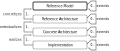
\includegraphics{figures/model-implementation-hierarchy}
  \caption{
    The hierarchical levels comprising the steps from a reference model to a software implementation.
    This document specifies a reference model only.
  }
  \label{fig:model-implementation-hierarchy}
\end{figure}

By implication, this document is not concerned with dictating how any of the concepts it defines relate to any \textit{protocols}, \textit{profiles}, \textit{specifications} or \textit{standards}, where a \textit{protocol} is understood to be a pattern of communication, a \textit{profile} to be a description of how a protocol is applied, a \textit{specification} to be a set of design constraints and, finally, a \textit{standard} to be a protocol, profile or specification ratified by a standards body.

\newpage

\subsection{Notational Conventions}
\label{sec:introduction:conventions}

\subsubsection{Diagrams}

Boxes with names inside them denote arbitrary entities.
A named arrow denote the relationship implied by its name.
A box being inside another box means that it is owned by the containing box.
See Figure \ref{fig:model-implementation-hierarchy} for an example of this graphical notation being used.

Note that this document does \textit{not} define an Arrowhead profile for SysML \cite{omg2019sysml}, or any other modelling language.
The concepts outlined here should corrsepond to the entities and relations defined by any such profiles, however.

\subsubsection{References}

Square brackets around numbers (e.g. \cite{delsing2017iot}) are references to the reference list in Section \ref{sec:references}.
The number within the brackets of any given reference corresponds to the entry with the same number in the reference list.

\subsubsection{Requirements}

Use of the words \textbf{must}, \textbf{must not}, \textbf{required}, \textbf{should}, \textbf{should not}, \textbf{recommended}, \textbf{may}, and \textbf{optional} are to be interpreted as follows when used in this document: \textbf{must} and \textbf{required} denote absolute requirements that must be adhered to for a described entity to be considered as compliant to this reference model; \textbf{must not} denotes an absolute prohibition; \textbf{should}, \textbf{should not} and \textbf{recommended} denote recommendations that should be deviated from only if special circumstances make it relevant; and, finally, \textbf{may} and \textbf{optional} denote something being truly optional.
These word definitions are derived from and are meant to capture what is outlined in RFC 2119 \cite{bradner1997keywords}.

\subsection{Relationships to Other Documents}
\label{sec:introduction:relationships}

The reference model outlined in this document is based on the following works, in order of precedence:

\begin{enumerate}
\item \textit{Reference Architecture Model Industrie 4.0} (RAMI4.0) \cite{adolphs2016reference}.
The model provides a ontological and architectural view of Industry 4.0, which makes it highly relevant to the Arrowhead framework.
As RAMI4.0 is a reference \textit{architecture} rather than a reference \textit{model}, however, its 5\textsuperscript{th} section is disregarded and its remaining sections treated as if being a reference model.
This delimitation excludes the ``architectural layers'', ``life-cycle \& value-stream'' phases and ``hierarchical levels'' of RAMI4.0.

\item \textit{Reference Model for Service Oriented Architecture} (SOA-RM) \cite{mackenzie2006reference}.
This standard has come to underpin many key trends within software engineering, such as cloud computing and microservices.
Service-oriented architecture is explicitly designated as an ontological foundation of RAMI4.0, which gives SOA-RM an indirect relationship to this document.

\item \textit{Prior work directly concerned with Arrowhead}.
This significantly includes \textit{IoT Automation: Arrowhead Framework} \cite{delsing2017iot}, which was written to provide a comprehensive overview of the framework.

\end{enumerate}

You are not assumed to have read any of the above documents prior to reading this.
Concepts derived from the above sources are reiterated in this document as necessary.

\subsection{Section Overview}
\label{sec:introduction:sections}

\begin{itemize}[leftmargin=3cm,rightmargin=0pt,labelwidth=2cm,labelsep=0pt,itemindent=0pt,parsep=0.25cm,topsep=0.25cm,align=left]

%\item[Section \ref{sec:introduction}]
%This section.

\item[Section \ref{sec:arrowhead}]
An informal overview of Arrowhead, serving both to provide a workable summary of the framework and to prepare readers for better understanding Section \ref{sec:model}.

\item[Section \ref{sec:model}]
The formal and normative description of Arrowhead.

\item[Section \ref{sec:conformance}]
A brief list of requirements, meant to help determine whether or not a given system is conforming to this document.

\item[Section \ref{sec:references}]
Lists references to publications referred to in this document.

\item[Section \ref{sec:revision}]
Records the history of changes made to this document.

\end{itemize}
